\documentclass[traditabstract]{aa}
%\documentclass[traditabstract, referee]{aa}

\usepackage[stable]{footmisc}
\usepackage{graphicx}
\usepackage[varg]{txfonts}
\usepackage{hyperref}
\usepackage{natbib,twoopt}
\usepackage{lscape}
\usepackage{hyperref} 
\usepackage{subcaption}
\usepackage{nicefrac}
\bibpunct{(}{)}{;}{a}{}{,} 

\makeatother\bibpunct[, ]{(}{)}{;}{a}{}{,}

\bibliographystyle{./bibtex/aa}

\newcommand{\farc}{\hbox{$.\!\!^{\prime\prime}$}} 
\newcommand{\ergA}{$\rm{erg\,c m^{-2}\,s^{-1}\,\AA\,^{-1}}$} 
\newcommand{\erg}{$\rm{erg\,cm^{-2}\,s^{-1}}$} 
\newcommand{\kms}{$\rm{km\,s^{-1}}$}
\newcommand{\hb}{H$\beta$} 
\newcommand{\ha}{H$\alpha$}
\newcommand{\hg}{H$\gamma$} 
\newcommand{\hd}{H$\delta$} 
\newcommand{\hi}{\mbox{H\,{\sc i}}} 
\newcommand{\hii}{\mbox{H\,{\sc ii}}} 
\newcommand{\ebv}{$E_{B-V}\,$} 
\newcommand{\oh}{12+\log(\mathrm{O/H})}

\newcommand{\hei}{\ion{He}{i}} 
\newcommand{\oi}{[\ion{O}{i}]} 
\newcommand{\sii}{[\ion{S}{ii}]} 
\newcommand{\siii}{[\ion{S}{iii}]} 
\newcommand{\oii}{[\ion{O}{ii}]}
\newcommand{\cii}{[\ion{C}{ii}]} 
\newcommand{\oiii}{[\ion{O}{iii}]}
\newcommand{\neiii}{[\ion{Ne}{iii}]}
\newcommand{\nii}{[\ion{N}{ii}]} 
\newcommand{\Msun}{$M_\odot$}
\newcommand{\Msunyr}{$M_\odot\,\rm{yr}^{-1}$}
\newcommand\nodata{ ~$\cdots$~ }

\begin{document}
\title{The super-massive black hole coincident with the luminous transient ASASSN-15lh\thanks{Based on observations at ESO, Program IDs: 097.D-1054, 297.B-5035}}

\titlerunning{A super-massive black hole coincident with the most luminous transient ASASSN-15lh.}

\author{Some people at some place}

\institute{Max-Planck-Institut f\"{u}r extraterrestrische Physik, Giessenbachstra\ss e, 85748 Garching, Germany
\and Institute of Astronomy, University of Cambridge, Madingley Road, Cambridge CB3 0HA, UK 
\and Department of Particle Physics and Astrophysics, Weizmann Institute of Science, Rehovot 7610001, Israel 
\and Dark Cosmology Centre, Niels Bohr Institute, University of Copenhagen, Juliane Maries Vej 30, 2100 K\o benhavn \O, Denmark 
}

\abstract{}


\keywords{}
\maketitle

\section{Introduction}
\label{sec:Intro}

One of the most curious astronomical transients reported in the recent year was arguably the object named ASASSN-15lh at a redshift of $z=0.233$, originally discovered by the All-Sky Automated Survey for Supernovae \citep[ASAS-SN][]{2014ApJ...788...48S} on 2015-06-24 \citep{2015ATel.7642....1N}. ASASSN-15lh is characterized by an exceptional brightness at peak ($M_u\sim23.5$~mag), high black-body temperatures over a long period (between $12\,000$~K and $25\,000$~K in the first 300 days) and relatively fast variability timescale of few tens of days. Its large radiated energy ($E_{\rm rad}\sim2\times10^{52}$~erg), rapid temporal evolution, a strong rebrightening at 120 days \citep{2016ApJ...828....3B}, and largely featureless optical spectra \citep{2016Sci...351..257D, 2016NatAs...1E...2L} make ASASSN-15lh hard to classify into the established scheme of transient phenomena, and have been used explore the diversity of existing theoretical models \citep{2015MNRAS.454.3311M, 2016ApJ...817L...8B}.

ASASSN-15lh was initially claimed \citep[][]{2016Sci...351..257D, 2017MNRAS.466.1428G} to be a hydrogen-poor Super-Luminous SuperNova (SLSN), an explosive phenomena from the collapse of a massive star \citep{2011Natur.474..487Q}, but other authors disagree with this classification \citep{2016NatAs...1E...2L,  2017ApJ...836...25M}. They argue that the observations are more consistent with a Tidal-Disruption Event \citep[TDEs, e.g.,][]{2015JHEAp...7..148K}, the luminous emission from the disruption of stars and fall-back accretion to the super-massive black hole in the center of galaxies \citep{1988Natur.333..523R, 1989ApJ...346L..13E}. This possibility was dismissed initially, primarily because the mass of black-hole $M_\bullet$ in the center of the galaxy that hosted ASASSN-15lh seemed too high \citep{2015ATel.7776....1P}: above $M_\bullet\sim10^{8}$~\Msun, the tidal radius of a solar-mass star lies within the Schwarzschild radius of a non-rotating black hole, and no radiation will escape these kind of encounters \citep{1975Natur.254..295H}.

The fundamental shortcoming of SLSN-related models stem from three independent observations: The absence of broad metal absorption lines that are typically observed in SLSN in their optical spectra. One of the most salient features in early SLSN spectra, for example, is related to an \ion{O}{ii}-doublet at 4100~\AA~and 4400~\AA \citep{2011Natur.474..487Q}. An absorption line at the corresponding wavelength of the bluer \ion{O}{ii} transition is detected, however, this would predict absorption by the redder transition \citep{2016MNRAS.458.3455M}, which would be much stronger than the limits implied by the available spectra \citep{2016NatAs...1E...2L, 2017ApJ...836...25M}. The temporal evolution of the transient would be unprecedented for SLSN, and its temperature and bolometric luminosity are inconsistent with previous observations of SLSN and the theoretical expectation of an expanding photosphere for these events. Last, the galactic environment of ASASSN-15lh is in stark contrast to previous hydrogen-poor SLSN hosts, which have exclusively been highly star-forming and of low-stellar mass and metallicity \citep{2015MNRAS.449..917L, 2016ApJ...830...13P, 2016arXiv160504925C}.

The physical properties of galaxies observed to host TDEs are in stark contrast to those of SLSN. They exhibit a curious preference  \citep{2014ApJ...793...38A, 2016ApJ...818L..21F} for E+A galaxies \citep{1996ApJ...466..104Z}. These galaxies are dominated by the stellar light from A-type stars, and show characteristic and strong Balmer absorption. They are thought to be the result of a star-burst several hundred million years in the past, possibly triggered my a galaxy merger \citep{1996ApJ...466..104Z}. In fact, the nearby TDE ASASSN-14li shows distinctive tidal tails in ionized gas emission, the result of a recent merger and ionization from an active galactic nucleus (AGN) in spatially-resolved spectrosopy \citep{2016ApJ...830L..32P}.

Because of the strong differences in the physical properties of the host galaxies of SLSN and TDEs, and the strong constraints that the environment can imply for the nature of the transient, we have obtained sensitive medium-resolution and spatially resolved spectroscopy of the field of ASASSN-15lh. These observation are pinpointing the exact position within the host, reveal emission lines from ionized hydrogen and metal lines, constrain the mass of the central black-hole and probe the large-scale environment.

Throughout the paper, we adopt a flat $\Lambda$CDM cosmology with Planck parameters ($H_0=67.3\,\mathrm{km}\,\mathrm{s}^{-1}\,\mathrm{Mpc}^{-1}$, $\Omega_\mathrm{m}$=0.315, $\Omega_\Lambda$=0.685, \citealt{2014A&A...571A..16P}), a \citet{2003PASP..115..763C} initial mass function (IMF), and report errors at the 1~$\sigma$ confidence level.

\section{Observations and data analysis}
\label{sec:Obs}

\subsection{Hubble Space Telescope imaging}
\label{obs:hst}


\begin{figure*}
  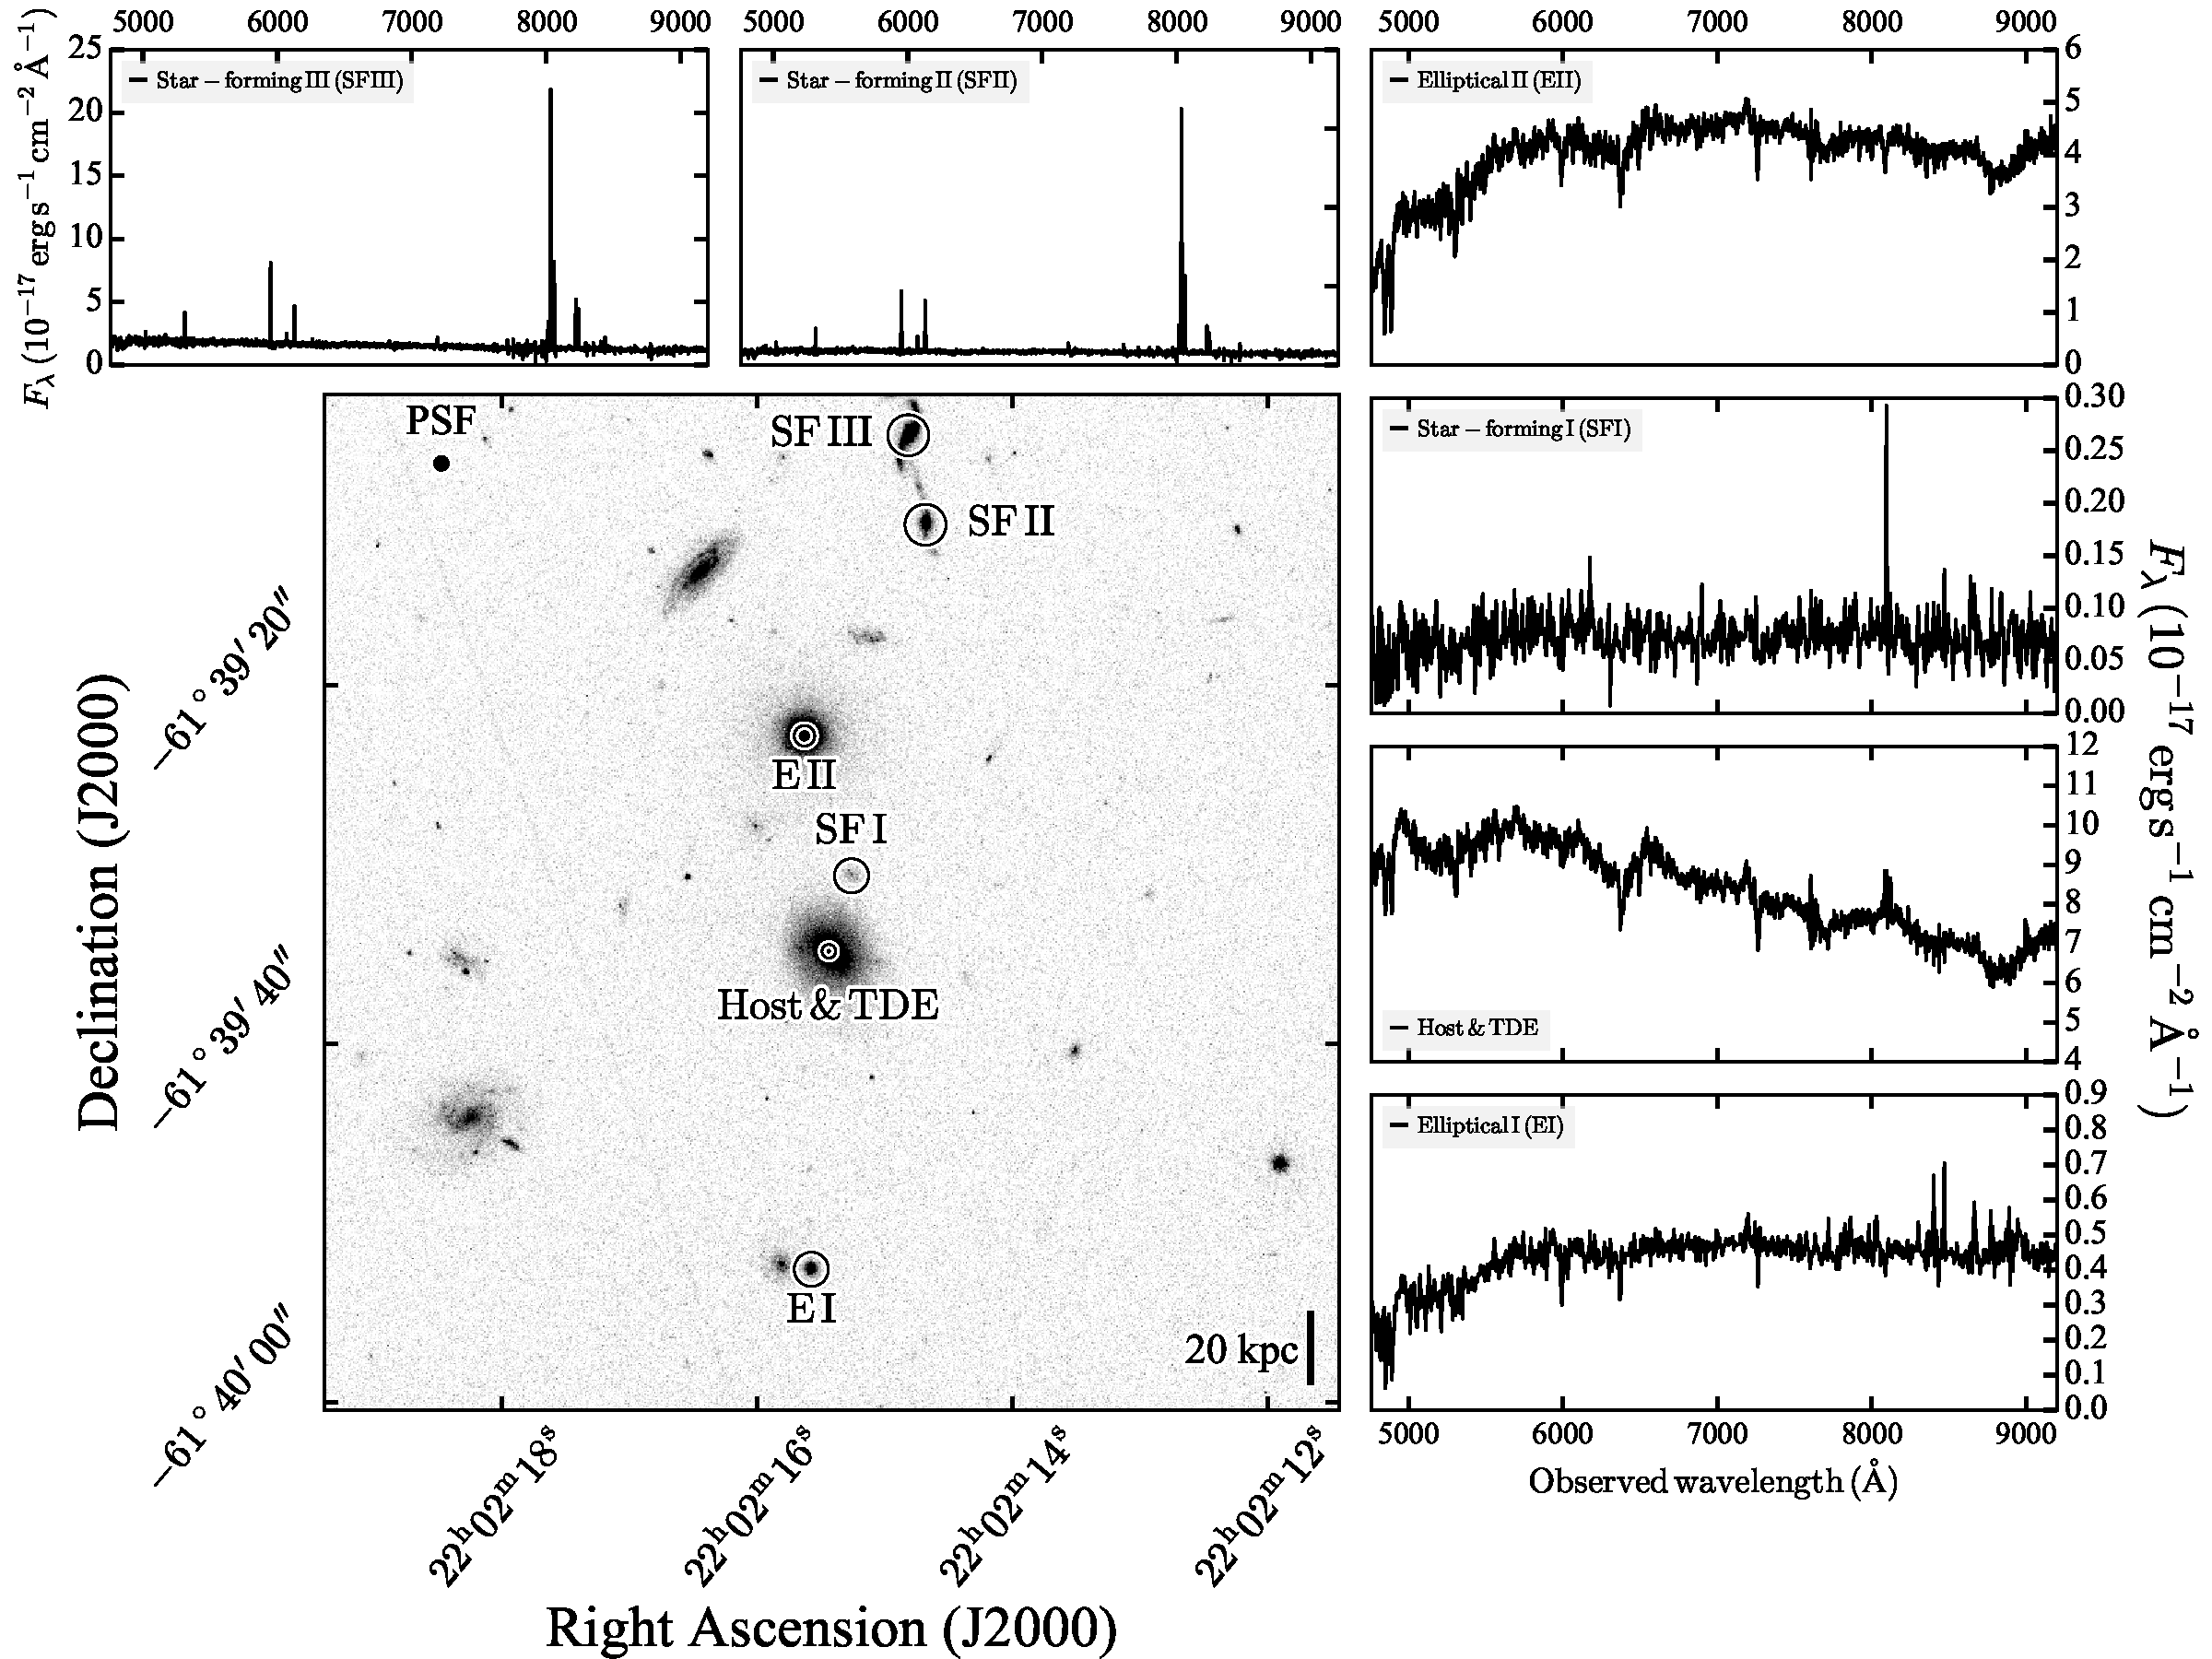
\includegraphics[width=0.999\linewidth]{fig/MUSE_ASASSN-15lh_wfc.pdf}
\caption{HST WFC3 image in the $F606W$ filter in the \textit{central panel}. The image spans approximately 60" by 60", which is 220 by 220~kpc at the redshift $z=0.233$ of ASASSN-15lh and corresponds to the field-of-view of our MUSE integral field spectroscopy (Section~\ref{obs:muse}). The six panels above and right of the WFC3 image show extracted MUSE spectra of the host (plus transient) as well as five additional galaxies at a similar redshift. These galaxies are marked SFI, SFII, and SFIII for the three star-forming galaxies as well as EI and EII for two ellipticals in the main image. The size of the MUSE PSF, as well as a physical scale at $z=0.233$ are indicated in the top left, and bottom right corner of the image respectively.}
\label{fig:fc}
\end{figure*}

The Hubble Space Telescope (HST) observed the field of ASASSN-15lh with the Wide-Field Camera 3 (WFC3) under program 14346 PI: C. Kochanek. A total of six exposures of 416~s integration time each was obtained on 2016-08-11 in the $F606W$ filter through Directors Discretionary Time and made public in the HST archive. We download the processed and CTE-corrected data and drizzle them onto a single frame with a pixel scale of 0\farc{025}\,$\mathrm{px}^{-1}$ or 93\,pc\,px$^{-1}$ at the redshift of ASASSN-15lh. The transient is clearly detected at high significance as a bright point-source (FWHM = 0\farc{07}) above the continuum emission of the galaxy. Tying the WFC3 astrometry to ten sources from the Gaia DR1 catalog \citep{2016A&A...595A...2G, 2016A&A...595A...1G}, we measure a position of $\mathrm{R.A.~(J2000)}=$22:02:15.4263, $\mathrm{Decl.~(J2000)} = -$61:39:34.910 in the astrometric reference frame defined by Gaia. The positional uncertainty is dominated by the root-mean-square difference to the astrometric tie-objects, which is 8 mas in each coordinate (30 pc co-moving). A cut-out from this image with a size of 1\arcmin\,by 1\arcmin and centered around the transient position is shown in the central panel of Figure~\ref{fig:fc}.

The HST imaging also shows the host to be elongated along the North-East, South-West direction, and together with the lack of recent star-formation and broad-band photometric colors, shows the typical characteristics of lenticular, or S0, galaxies \citep[e.g.,][]{2009ARA&A..47..159B}. Within hierarchical structure formation, lenticular galaxies are often thought to be the result of mergers in particular in group environments where galaxy encounters are frequent \citep[e.g.,][]{2005A&A...437...69B, 2011MNRAS.415.1783B}. However, other physical processes like ram pressure stripping or quenching of spirals due to starvation could play a role as well, so that the formation of S0s remains the subject of active study.


%QFitsview centroid from the astrometrized image.

\subsection{VLT/X-Shooter long-slit spectroscopy}
\label{obs:xs}

We initiated ground-based observations of ASASSN-15lh with X-Shooter \citep{2011A&A...536A.105V}, a cross-dispersed long-slit spectrograph mounted at ESO's Very Large Telescope (VLT) Unit Telescope (UT) 2. X-Shooter operates in three arms, simultaneously covering the wavelength range of $3000$\,AA\,to $25\,000$\,\AA\, with a resolution between 30\,\kms\, and 60\,\kms\, depending on the slit width and arm. In total, we obtained approximately 5700~s of integration split over two nights (2016-07-02 and 2016-08-02) through program 297.B-5035 (PI: M. Fraser). We used X-Shooter slits widths of 1\farc{0} (3000\AA\,to 5500\,\AA), 0\farc{9} (5500\,\AA\,to 10\,000\,\AA) and  0\farc{9} (10\,000\,\AA to 25\,000\,\AA) respectively, which were centered at the transient and oriented along the parallactic angle. Given that the transient aligns with the brightest part of the galaxy, these spectra are hence a superposition of transient and galaxy light.

The X-Shooter spectroscopy was reduced in a similar manner as described in detail in \citet{2015A&A...581A.125K}, making use of the ESO pipeline in its version \texttt{2.7.1} \citep{2006SPIE.6269E..80G, 2010SPIE.7737E..56M} and self-written methods and tools. The data were flux-calibrated against the nightly spectra-photometric standard, which was LTT7987 on 2016-07-02 and EG274 on 2016-08-02, and extracted using variance-weighting. The signal-to-noise of the final spectrum is between 20 and 30 per spectral bin of size 0.4\,\AA\,in the observed wavelength range 3800\,\AA\, to 9700\,\AA\, and somewhat lower above and below.

\subsection{VLT/MUSE integral-field spectroscopy}
\label{obs:muse}

We also used the Multi-Unit Spectroscopic Explorer (MUSE, \citealt{2010SPIE.7735E..08B}) at VLT UT4 to obtain spatially-resolved spectroscopy of the field around ASASSN-15lh. MUSE is a state-of-the-art integral field unit (IFU) with an unprecedented combination of sensitivity, spatial sampling (spaxel size of 0\farc{2}\,x\,0\farc{2}), wavelength coverage (4750\,\AA\,to 9350\,\AA) and resolving power ($R=1500$ to $R=3000$ increasing from blue to red wavelengths). Similar to our X-Shooter data (Section\,\ref{obs:xs}), we tried to obtain IFU spectroscopy in two epochs (2016-08-11 and 2016-08-26). However, observations during the first date were carried out by ESO under adverse conditions such that they are practically useless for our purpose. We are hence left with a total of 3600\,s of MUSE spectroscopy from 2016-08-26, which was obtained under program 097.D-1054 (PI: S. Kim). The VLT/MUSE PSF of this epoch then defines the effective spatial resolution and has a FWHM of 0\farc{8} at 8000\,\AA.

Initial data processing was performed via the MUSE pipeline\footnote{http://www.eso.org/sci/software/pipelines/} (version \texttt{1.6.2}, \citealt{2014ASPC..485..451W}), which produces a fully reduced and sky-subtracted data cube, that has been calibrated in wavelength, flux and astrometry. Starting with this pipeline-produced data cube, we use third-party software to correct for telluric absorption (\texttt{molecfit}, \citet{2015A&A...576A..77S}) as well as sky-line residuals (\texttt{ZAP}, \citealt{2016MNRAS.458.3210S}).

We further correct the MUSE flux-scale through synthetic photometry of the star at $\mathrm{R.A.~(J2000)}=$22:02:11.92, $\mathrm{Decl.~(J2000)} = -$61:39:46.6 (Figure~\ref{fig:fc}) and comparison to its $r$- and $i$-band magnitudes from \citet{2016NatAs...1E...2L}. To map the accurate, HST-derived position from Section~\ref{obs:hst} onto the MUSE data cube, we first reconstruct several images centered at various wavelengths from the MUSE integral field spectroscopy. The MUSE field-of-view contains a handful (5-7) of comparison stars which we can then use to register the MUSE astrometry against the HST imaging using a linear transformation\footnote{The optical distortion of MUSE, visible as a trapezoidal shape of the field of view is already calibrated out of the data cube through the   astrometric solution applied by the MUSE pipeline.}. The registration of different re-constructed images yields consistent results within a typical scatter smaller than 40 mas (or 0.2 MUSE pixels). This places ASASSN-15lh in our MUSE data cube data with a total accuracy better than 150 pc in each coordinate.

\section{Results}
\label{sec:Res}

\subsection{Modeling the spectral continuum}

\begin{figure}
  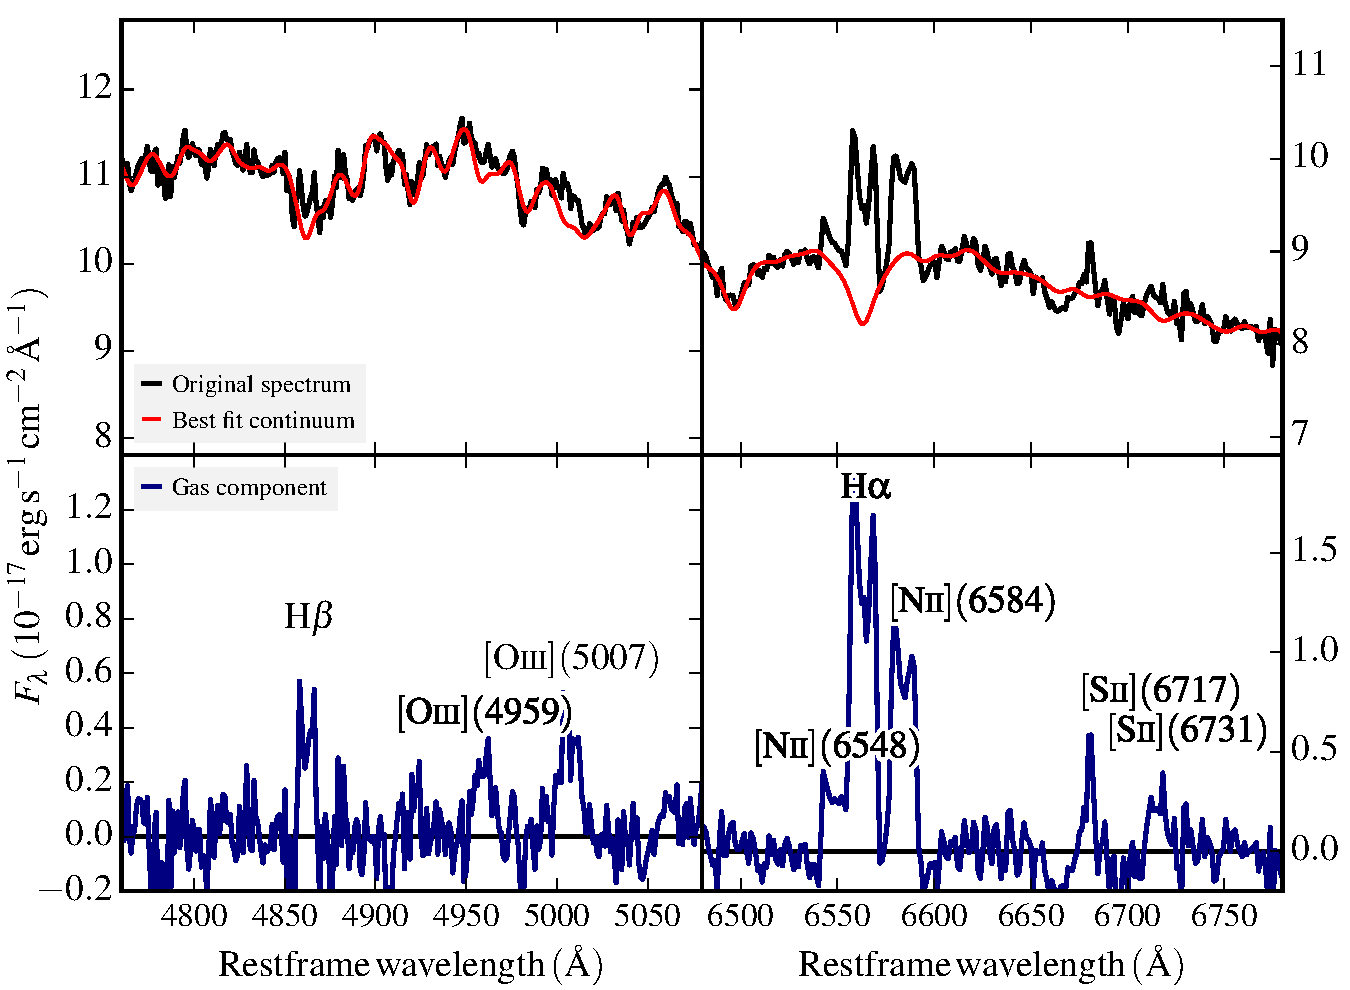
\includegraphics[width=0.999\linewidth]{fig/MUSE_stargas.pdf}
\caption{Decomposition of continuum and gas emission. The \textit{upper two panels} shows the spectrum}
\label{fig:stargas}
\end{figure}

Fluxes from strong emission lines due to the recombination of Hydrogen and decay of collisionally-excited states of metal ions provide information on the physical properties of the plasma, as well as its ionization source. In particular the Balmer lines, however, are a superposition of stellar absorption lines, emission lines of the ionized gas and a potential contribution of the transient itself. 

We try here to disentangle these different components by modeling the observed continuum with stellar templates and emission from the transient represented with a low-order polynomial. An illustrative example of this procedure using penalized pixel fitting \citep[pPXF,][]{2004PASP..116..138C, 2017MNRAS.466..798C} is given in Fig.~\ref{fig:stargas}.

Here, we show the spectrum central component of the host extracted from the MUSE cube to illustrates already a couple of noteworthy observations. Firstly, there are obvious detection of multiple emission lines, which correspond to the transitions of \hb, \oiii($\lambda\lambda$4959, 5007), \nii($\lambda\lambda$6548, 6584), \ha\, and potentially \sii($\lambda\lambda$6717, 6731), even tough the significance of the latter is not particularly convincing and depends somewhat on the details of the subtraction. Secondly, each of these lines is clearly not well described with a Gaussian and shows velocity structure. We will return to the line shape and discuss it in detail in Sect.~\ref{sec:prof}.

\subsection{The central stellar population}
\label{sec:spop}

To derive a more physical interpretation of the continuum, we used simple black-body fits for the transient in combination with galaxy templates from stellar populations synthesis models to fit to our spectroscopy. These fits, however, turned out to be unsatisfactory to accurately disentangle emission lines from the continuum as they returned strong, broad residuals in the subtracted spectrum. These are likely deviations of the ASASSN-15lh spectrum from a pure black-body, as similar fits to spectra of EI (Fig.~\ref{fig:fc}) show no residuals. Here, we used \texttt{starlight} \citep{2005MNRAS.358..363C, 2009RMxAC..35..127C} and \citet{2003MNRAS.344.1000B} templates in a similar manner as we have described in detail elsewhere \citep{2016MNRAS.455.4087G, 2017arXiv170205430K}.

The details of the stellar continuum model vary somewhat depending on the exact choice of the size of the spectral extraction, the best-fit transient black-body temperature, as well as the base list of galaxy templates. However, contributions from two stellar populations are always required for a decent fit of the stellar component in the galaxy center: a population with an age of around 1~Gyr to 2~Gyr, another one that is significantly older with an age of 10~Gyr to 13~Gyr. Previously estimated ages of around 5~Gyr from pre-explosion broad-band photometry \citep{2015ATel.7843....1M, 2016NatAs...1E...2L,  2016Sci...351..257D} can then be explained by a superposition of the two spectroscopic components. 

\subsection{Stellar kinematics and mass of the central black hole}

\begin{figure}
  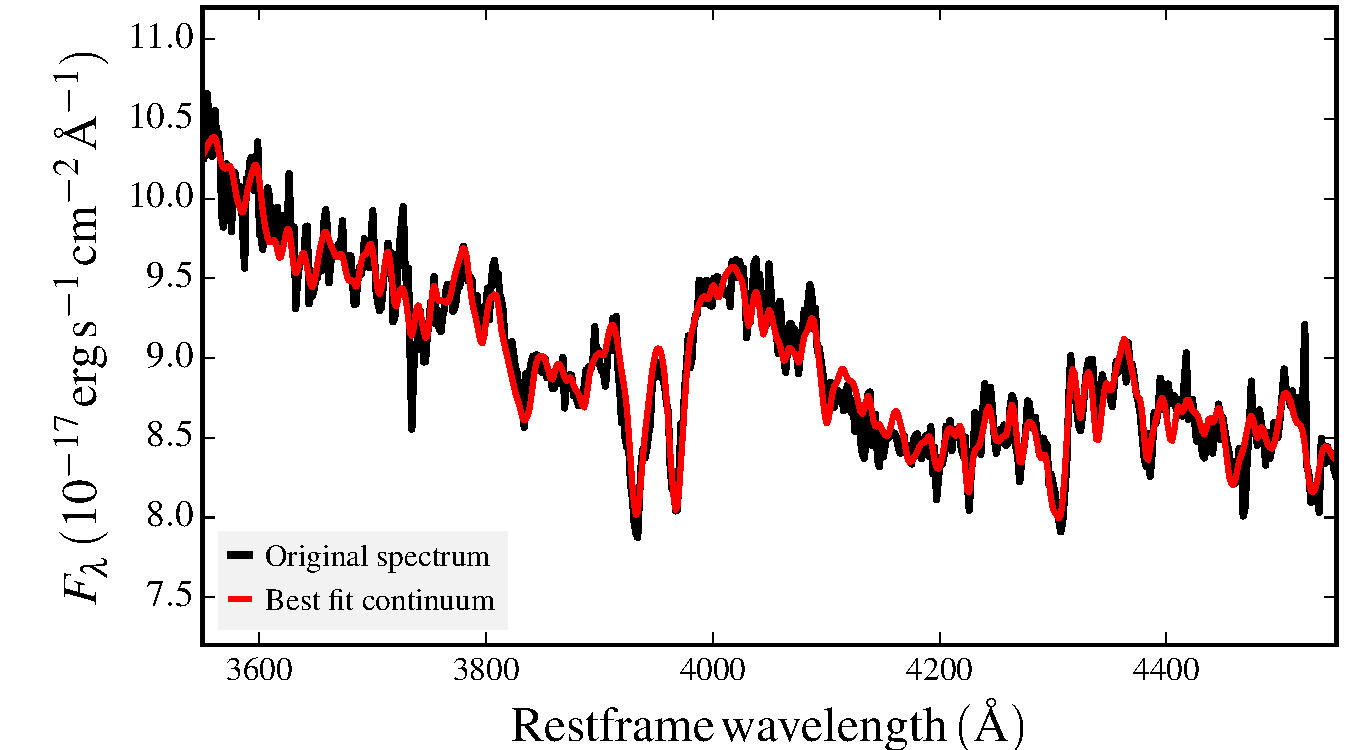
\includegraphics[width=0.999\linewidth]{fig/XS_stargas.pdf}
\caption{Stellar continuum fit for determination of stellar kinematics. The emission from the transient is clearly evidence as the continuum is bluer than what would be expected form the host galaxy alone.}
\label{fig:stargas_sig}
\end{figure}

A similar fit as in the previous sections also returns the stellar kinematics, and in particular velocity dispersion of the stellar component ($\sigma$). Figure~\ref{fig:stargas_sig} shows the medium resolution X-shooter spectrum (Instrumental resolution $\sigma_{\mathrm{inst}}=25$\,\kms) in the wavelength range of the strong \ion{Ca}{II}~H+K doublet, \hd, \hg, and the G-band, as well as the best fit continuum which results in a central velocity dispersion of $\sigma=225\pm15$\,\kms. This value corresponds to a mass $M_\bullet$ of the central black hole of $M_\bullet = 5.3_{-3.0}^{+8.0}\cdot10^{8} M_\sun$ \citep[Eq. 3, 5 or 7 in][]{2013ARA&A..51..511K}, where the largest part of the uncertainty comes from the intrinsic scatter in the $M_\bullet$-$\sigma$ relation ($\sim0.3$\,dex). The Eddington luminosity for this black hole mass is $L_{\mathrm{Edd}}=6.7_{-3.8}^{+10.1}\cdot10^{46}$~erg~s$^{-1}$.

%\subsection{Large-scale Environment}

\subsection{Emission-line profiles}
\label{sec:prof}

\begin{figure}
  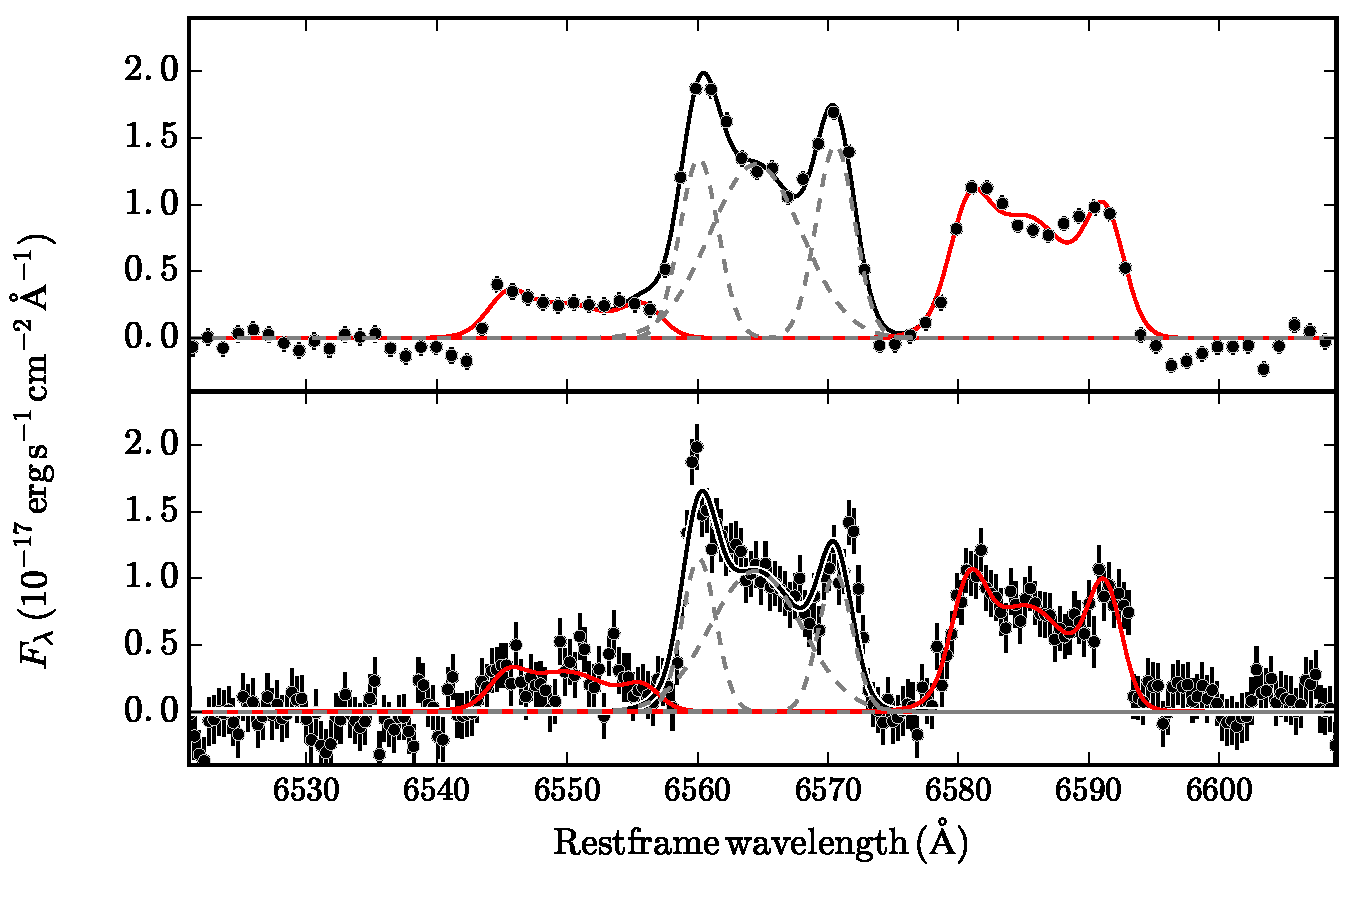
\includegraphics[width=0.999\linewidth]{fig/MUSE_XS_lineshape.pdf}
\caption{Emission-line profiles for the \ha\, and \nii\, complex. A spectrum extracted for the central component of the host galaxy from the MUSE datacube}
\label{fig:hanii}
\end{figure}

Now that the continuum from stars and transient has been separated from the emission lines, we look more closely to the line shape and velocity structure of the \ha\, and \nii\, complex of Fig.~\ref{fig:stargas} in order to study the ionization source, and their relation to the transient.

In Fig.~\ref{fig:hanii} shows a zoom-in to the continuum-subtracted wavelength range of the respective transitions from our MUSE and X-shooter spectroscopy. The line-shape of the individual transitions is complex, and consists of three components that are well-separated in wavelength space - a central, broader component (FWHM=8\,\AA~ or 380~\kms), as well as a narrower (FWHM=3\,AA~ or 100\,\kms) blue and red component offset by approximately 5\,\AA~ (250~\kms) in each direction. The line shape of the \ha\, and each of the collisionally excited \nii($\lambda\lambda$6548, 6584) appears identical within the measurement uncertainties. Also, the line shape is well-resolved, in particular through the medium-resolution X-shooter data, and appears comparable between the two spectrographs\footnote{The width of the instrumental resolution at the wavelength range of \ha~(observed 8100\,\AA) has a FWHM=110\,\kms~ for MUSE and a FWHM=35\,\kms~for X-Shooter.}.

The emission lines from the \hb~ and \oiii~ transitions are generally consistent with this picture (Fig.~\ref{fig:stargas}), in particular \hb~ shows evidence for a similar line-profile. However, large statistical errors stemming from the bright background and systematic uncertainties from the continuum subtraction prevent us from performing a detailed kinematic analysis for any other lines than \ha~and \nii.

To derive line-fluxes and gas kinematics, we fit a superposition of three Gaussians for each of the three transitions simultaneously to the spectra shown in Fig.~\ref{fig:hanii}. The intrinsic line-width, broadened by the instrumental resolution, is tied between both instruments and the three transitions, and only the normalization is allowed to vary during the fit. Table~\ref{tab:lines} contains the fit parameters and line-fluxes from this procedure.

\subsection{Positional analysis of the emission-line components}

\begin{figure}
\begin{subfigure}{.49\textwidth}
  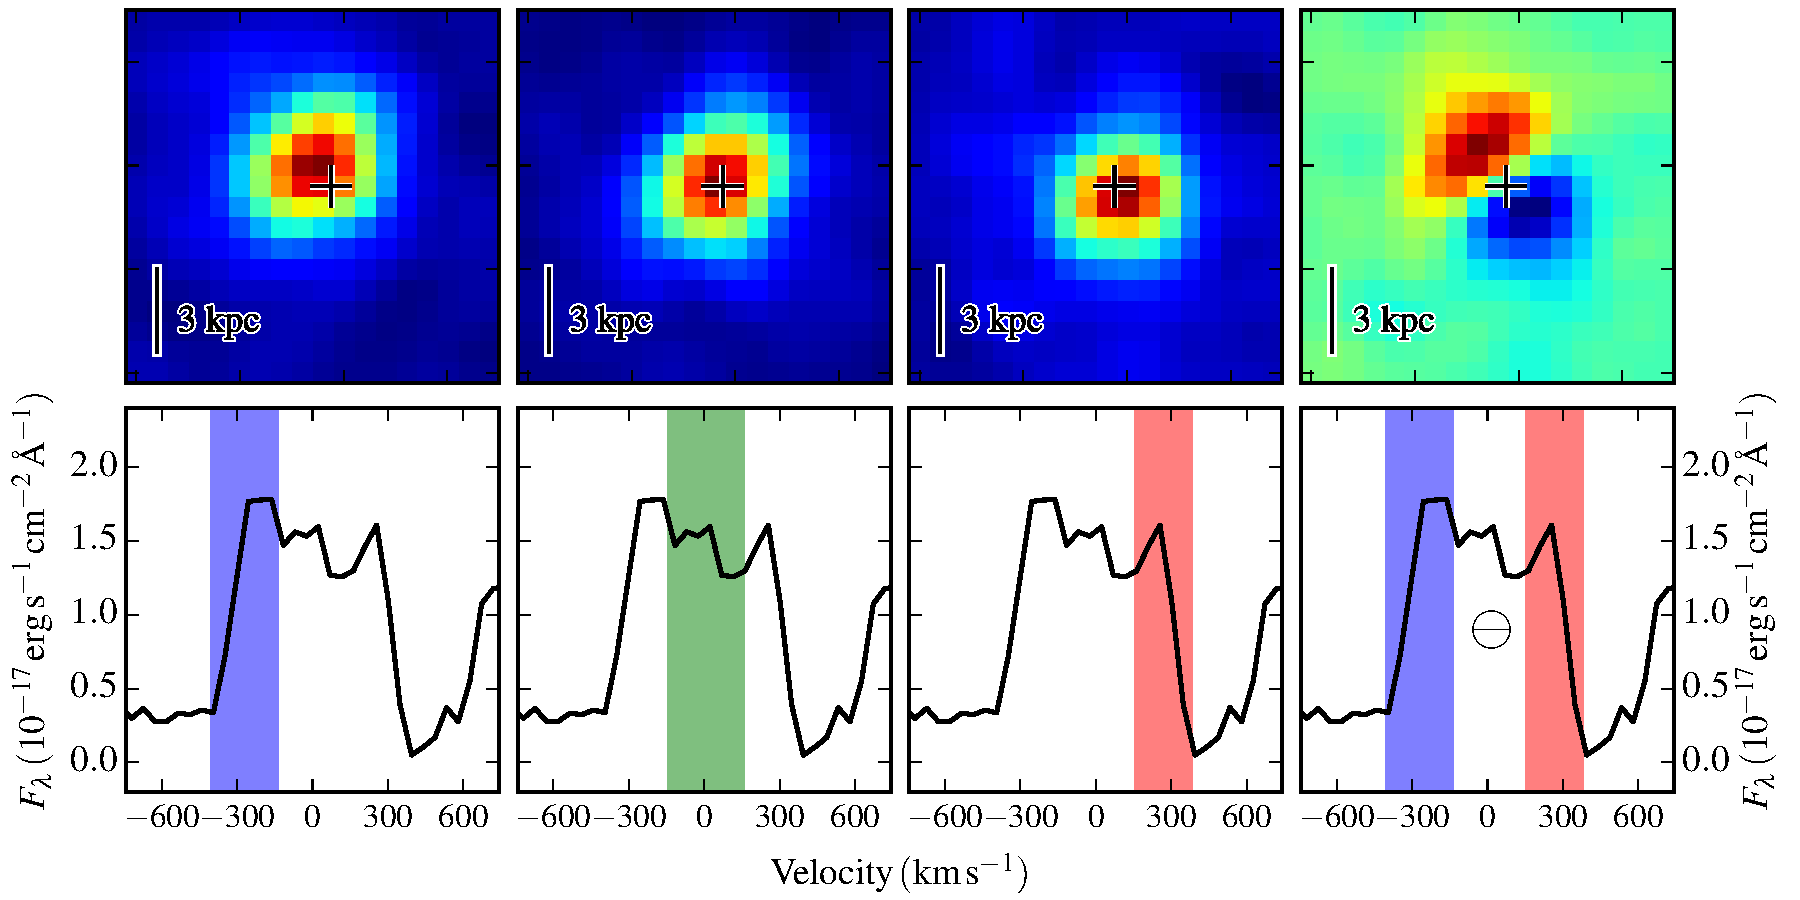
\includegraphics[width=0.999\linewidth]{fig/MUSE_Ha_channelmaps.pdf}
\end{subfigure}
\begin{subfigure}{.49\textwidth}
  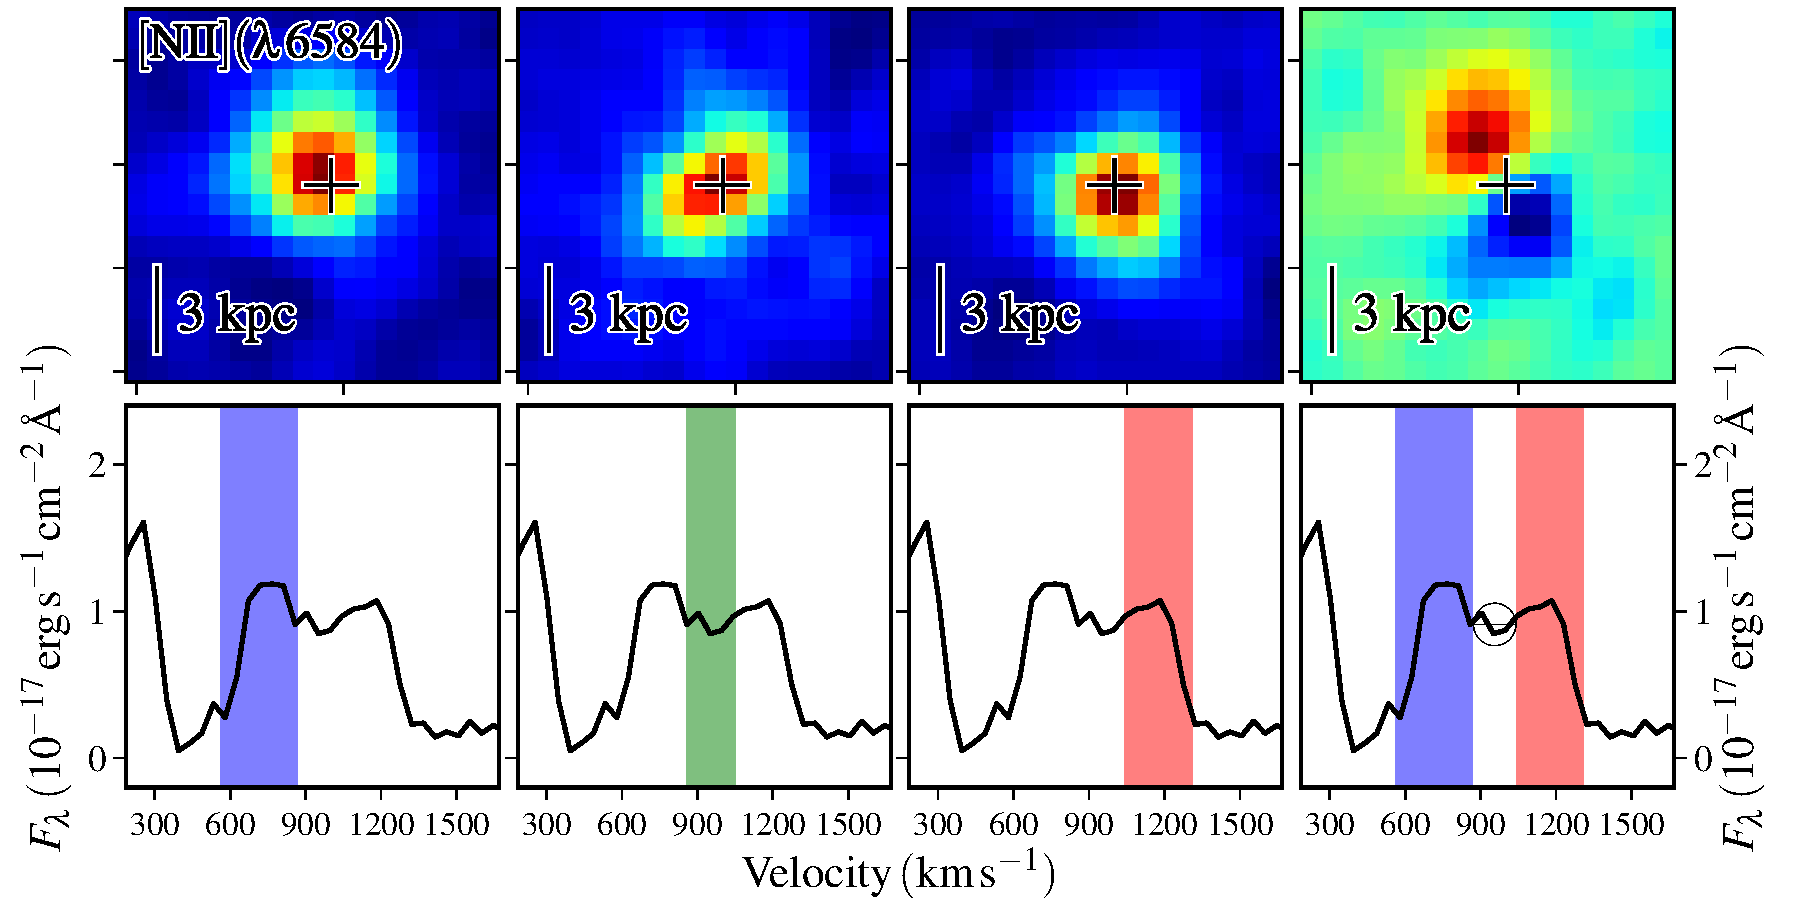
\includegraphics[width=0.999\linewidth]{fig/MUSE_NII_channelmaps.pdf}
\end{subfigure}

\caption{Channel maps of the velocity components. The two \textit{upper} rows show in the three leftmost panels the reconstructed images in a given velocity range from the continuum-subtracted MUSE map for \ha. The right panel shows a subtraction between the blue and red-components. The position of the transient is indicated by a cross. The two \textit{lower} rows show the same for \nii. All images have been smoothed by a 2x2 Kernel for illustration purposes. The physical scale of the images in indicated by the bar in the lower-left corner of each image. North is up, and East is left in all images.}
\label{fig:channelmaps}
\end{figure}

The MUSE integral-field spectroscopy allows us to go beyond a standard kinematic analysis as done above, and perform a spatially-resolved study of the individual velocity components. Here, we created a continuum-subtracted data cube from the original MUSE spectroscopy by performing a fit similar to the one of Fig.~\ref{fig:stargas}, but now for each individual spaxel in the astrometrically-calibrated data (Sect.~\ref{obs:muse}). Similar procedures have been used by us frequently in the past on MUSE data \citep{2016MNRAS.455.4087G, 2016ApJ...830L..32P, 2017arXiv170205430K}, and allow us to combine and visualize the spatial information of the MUSE maps with the velocity information of the emission line kinematics.

Figure~\ref{fig:channelmaps} shows the channel maps of the continuum-subtracted integral-field spectroscopy at the center of the transient host, and in the wavelength range of \ha. Each of the three panel shows the reconstructed image in the given wavelength range, whereas the rightmost panel is a subtraction between the bluest and reddest component. The position of the transient as derived through the HST-to-MUSE astrometrical alignment is indicated by a cross.

Its evident that the three velocity components are not only separated in velocity space, but are also placed at different positions. Both, blue and red components are further inconsistent with the transient location. The velocity separation between the blue and red component is 500~\kms, and the spatial offset is $1.8\pm0.3$ MUSE spaxel or $0\farc{36}\pm0\farc{06}$, corresponding to a projected distance of $1.3\pm0.2$~kpc.

The central velocity component is placed symmetrically between the red and blue components (both spatially, as well as in velocity space), and is consistent with the transient position within the combined astrometric uncertainty of $0.22$ MUSE spaxel, or 45 mas, which corresponds to a physical scale of 170 pc at $z=0.233$.

\subsection{Ionization source}
\label{sec:ionsource}

\begin{figure}
  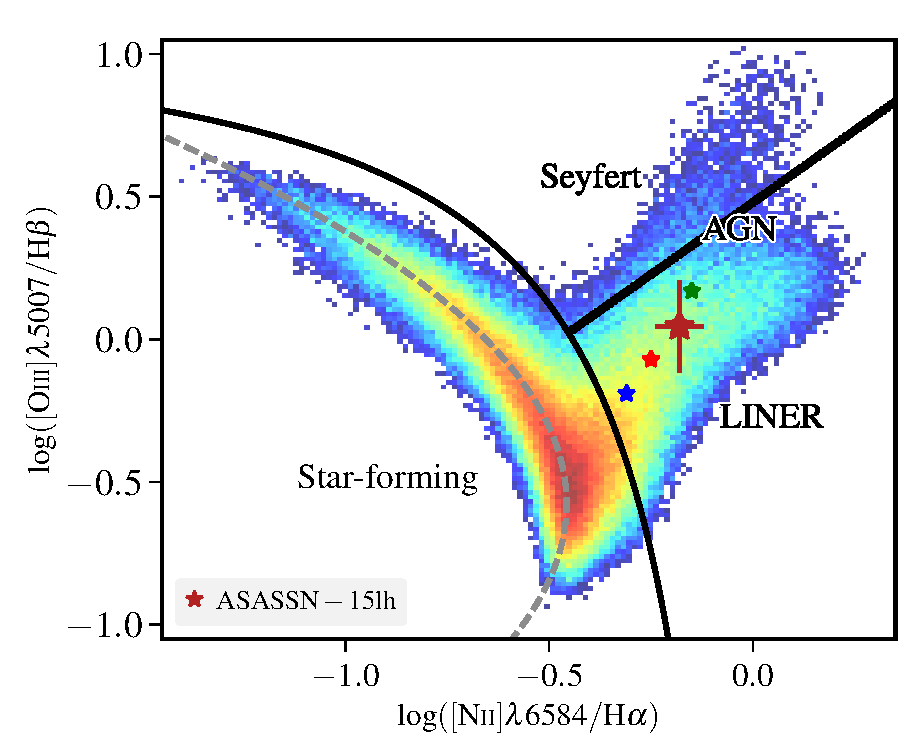
\includegraphics[width=0.999\linewidth]{fig/BPT.pdf}
\caption{The host of ASASSN-15lh in the BPT diagram. The large, red star represent the flux ratios of the total integrated line flux, while the three smaller stars the three individual components. The black solid lines are differentiation lines between star-forming galaxies and AGN of \citet{2013ApJ...774L..10K} at $z\sim0.23$, as well as LINER and Syfert differentiation lines from \citet{2010MNRAS.403.1036C}. The grey dashed line is the ridge line, i.e., the line with the highest density of star-forming galaxies \citep{2008MNRAS.385..769B}.}
\label{fig:BPT}
\end{figure}

The strength and ratios of various collisionally-excited and recombination lines trace the physical conditions in the gas-phase as well as the radiation that was ionizing the gas in the first place. A very popular diagnostic plot is the Baldwin-Phillips-Terlevich (BPT) diagram \citep{1981PASP...93....5B}, using the ratios of \nii/\ha~ and \oiii/\hb~ to discriminate between ionizing flux coming from the hard radiation of AGN or shocks or normal \hii~regions where the UV-flux is dominated by massive stars. 

The BPT diagnostic is frequently used for host galaxies of transient objects, and different classes of objects occupy very different phase-space. For example, the hosts of $\gamma$-ray bursts or super-luminous supernovae typically occupy the high \oiii/\hb, low \nii/\ha regime \citep{2015A&A...581A.125K, 2015MNRAS.449..917L}, characteristic of young starbursts at low metallicity. In contrast, the nearby ($d_L=90$~Mpc) TDE ASASSN-14li \citep{2016MNRAS.455.2918H} showed an extended structure of ionized gas with emission-line ratios that ascertain ionization from an AGN \citep{2016ApJ...830L..32P}.

The ionized regions of ASASSN-15lh are shown in the BPT diagram in Fig.~\ref{fig:BPT}, where we use the SDSS DR7 spectroscopy \citep{2009ApJS..182..543A} with line-fluxes from the MPA/JHU catalog as a background sample. It is evident that all components of the host, including the integrated flux of all components, are located in the part of the BPT diagram that is occupied by low-luminosity AGN and shock ionization/excitation.

In particular also the central component, which is positionally coincident with the transient, shows high values of \nii/\ha. These measurements of the line-ratios are inconsistent with ionization from only star-formation, but ascertains at least a large fraction of the ionization as coming from AGN or shocks \citep{2011MNRAS.413.1687C}. Similarly, a classification based on the equivalent width (EW) of \ha, as well as the \nii/\ha~ratio \citep{2011MNRAS.413.1687C} shows the ASASSN-15lh host to be consistent with a weak AGN (\nii/\ha~$>0.4$, and $3~\AA < \mathrm{EW}_{\mathrm{H}\alpha} < 6~\AA$), sometimes referred to as low-ionization nuclear emitting regions or LINERs.

The leading theoretical model to explain LINERs is photo-ionization from a central, low-luminosity AGN \citep[e.g.,][for a review]{2008ARA&A..46..475H}. In contrast to other ionization possibilities (young stars, fast shocks, evolved stars), a narrow-line region of a central AGN would naturally explain the line-ratios, the kinematics, and the spatial offsets between the three observed kinematic components.

We thus conclude that the line emission observed in ASASSN-15lh is most likely the radiation from gas photo-ionized by AGN radiation, and neither from star-formation nor the transient itself. The host is hence largely quiescent, being located 2-3 orders of magnitudes below the main sequence of star-forming galaxies.

Summing over all spectral components, the total \oiii~or \ha~luminosity is $L_{\oiii}\sim10^{40}$~erg~s$^{-1}$ or $L_{\mathrm{H}\alpha} \sim 3 \times 10^{40}$~erg~s$^{-1}$, respectively. These values correspond to an X-ray luminosity of around $L_{\mathrm{X}}\sim10^{41}$~erg~s$^{-1}$ in the 2-10 keV energy range, or a bolometric luminosity of $L_{\mathrm{bol}}\sim10^{42}$~erg~s$^{-1}$ to $L_{\mathrm{bol}}\sim10^{43}$~erg~s$^{-1}$ assuming average correction factors \citep{2008ARA&A..46..475H, 2009A&A...504...73L, 2012MNRAS.425..623L}. Even though these luminosity estimates are uncertain by at least an order of magnitude, the Eddington ratio $\lambda$ is far below unity ($\lambda\sim10^{-5}--10^{-4}$).

\section{Discussion}
\label{sec:Disc}

\subsection{The nature of the ionized-gas emission}

As shown in the previous paragraphs, the emission-line profiles observed in the ASASSN-15lh host galaxy nucleus is complex, and consists of multiple components with spatial and velocity offsets (Figures~\ref{fig:channelmaps}). The components are aligned along a single direction, and all are likely to be ionized by an AGN. Initially, the double-peaked nature of the \ha~ and \nii~line, lead us to suspect a binary AGN as origin of the emission. Giant early-type galaxies as the ASASSN-15lh host are thought to be the result of galaxy mergers in current galaxy formation theory \citep[e.g.,][and references therein]{2006ApJS..163....1H}. Because supermassive black holes (SMBHs) arguably reside in the centers of all massive galaxies \citep[e.g.,][for a review]{2013ARA&A..51..511K}, a good fraction of spheroidal galaxies should also host binary SMBH. If active, for example through nuclear accretion induced by the merger, the double SMBH will appear as a binary AGN. The most convincing cases of binary AGN on kpc scales, as would be the case here, are imaged as double point source in hard X-ray \citep[e.g.,][]{2003ApJ...582L..15K, 2008MNRAS.386..105B} or radio emission \citep{2011ApJ...740L..44F, 2015ApJ...813..103M}.

However, this scenario seems unable to fully explain our observation: while the line-shape from our MUSE data could conceivably be explained with two spectral components, the higher-resolution X-shooter data clearly demonstrates the presence of three components - the shoulder of the red and blue component are steep, so a symmetric emission profile always leaves residuals in the center (Fig. ~\ref{fig:hanii}). We would hence need to invoke three aligned and active SMBH, which we consider too contrived to explore further. We do note that only the medium-resolution X-shooter data (FWHM=30\,\kms) has allowed us to rule out this possibility. With the spectral resolution of MUSE (FWHM=150\,\kms) alone, we would have probably been mislead to consider a binary AGN origin for the line profile in more detail. 

Instead, we consider narrow-line gas kinematics, or galactic winds driven by the AGN a much more natural explanation for the observed kpc-scale emission in Balmer and collisional excited metal lines \citep[e.g.,][]{2011ApJ...735...48S}. Indeed, complex narrow-line regions (NRLs) are explained with AGN outflows at least for some nearby galaxies \citep[e.g.,][]{2011ApJ...727...71F} but the differentiation between rotating NLR disks and outflows not always trivial \citep{2011ApJ...735...48S, 2015ApJ...813..103M} in general. In our case, we observe a relatively symmetrical line-profile, as well as a geometry aligned along the major axis of the galaxy (), which both argues for an origin in a rotating disk of ionized gas. Clearly, the stellar population is much more extended than the emission lines, and it does not show strong sign of rotation in the core. Neither the red nor blue component of the emission lines has a kinematic counterpart to absorption lines observed in the stellar component. Hence, we are lead to suggest  that the emission line shape and position of all components is caused by a central AGN with a rotating disk of ionized gas, but clearly not multiple black holes on kpc scales.

The considerations above do not imply that there is not a binary black hole on much smaller, i.e., pc scales, and in fact we still consider it quite likely that such a binary black hole might be present. However, it seems clear that the observation of a complex line profile and kpc-scale emission of narrow lines is not the direct consequence of a binary AGN.

\subsection{Constraints on the origin of the transient}

Having pinpointed the location of the transient to the position of a weak AGN (and therefore a super-massive black hole), relating both of these phenomena seems reasonable. It thus leads us to constraints on the nature of ASASSN-15lh, with three different scenarios typically discussed in the pertinent literature \citep[e.g.,][]{2011ApJ...735..106D, 2014MNRAS.445.3263H, 2015ApJ...798...12V}: a very luminous core collapse supernova in the nuclear region of the host, a tidal disruption event or intrinsic variability from the AGN.

The first of those, a luminous supernova at the nucleus of a passive galaxy appears somewhat contrived for ASASSN-15lh in several ways: firstly, there are the inconsistencies of the spectral properties and temporal evolution of the transient with other SLSN or luminous SN of type IIn \citep{}. And secondly, the positional coincidence with a NLR of a quiescent galaxy strongly suggests that ASASSN-15lh is the result of a physical phenomenon closely related to the SMBH and not star-formation. 

AGN, and to some extend also quiescent SMBH such as the one in the center of the Milky-Way, are known to be variable on various time-scales and all wavelengths \citep[e.g.,][]{1997ARA&A..35..445U, 2001Natur.413...45B}. Typically, these forms of AGN variability are considered to be stochastic resulting from changes in the accretion rate, clearly not able to explain the ASASSN-15lh variability and spectral evolution. However, much more dramatic variations have been observed in changing-look quasars on shorter time-scales \citep[e.g.,][]{2014ApJ...788...48S, 2015ApJ...800..144L, 2017ApJ...835..144G}, even though also here the discrimination between AGN activity and TDEs is not always obvious \citep{2015MNRAS.452...69M}. Several lines of evidence indicate that such an AGN-related event is probably not the origin of ASASSN-15lh itself. Firstly, no strong X-ray variability for ASASSN-15lh is observed, despite regular monitoring and dramatic, simultaneous changes in the UV flux \citep{2016ApJ...828....3B, 2017ApJ...836...25M}. And secondly, also the optical-line emission is consistent with being constant throughout the last two years \citep{2016NatAs...1E...2L}, so that appearing broad lines or an increase in the continuum emission from a Syfert 1 would be readily detected.

In the light of our detailed observation of the transients environment, it thus seems to appear that the explanation of ASASSN-15lh as a TDE \citep{2016NatAs...1E...2L, 2017ApJ...836...25M} remains the most plausible one. TDEs within galaxies with regions of AGN ionization and excitation have been discovered before. ASASSN-14li is arguably the best-observed event \citep{2016MNRAS.455.2918H, 2016ApJ...830L..32P}, but a more recent candidate is reported in \citet{2017arXiv170307816B}. 

\subsection{The X-ray emission}

The detection of X-rays \citep{2017ApJ...836...25M} could provide important clues to the nature of the transient, however, it is also plausible that they originate from the AGN and are thus unrelated to ASASSN-15lh. Comparing our estimates of X-ray luminosity from the weak AGN with the measurements of \citet{2017ApJ...836...25M}, who estimate a 0.3-10~keV flux of $L_{\mathrm{X}}\sim10^{41}$~erg~s$^{-1}$ to $L_{\mathrm{X}}\sim10^{42}$~erg~s$^{-1}$. Given that this measurement is derived in a somewhat larger energy interval than our estimate of the hard X-ray flux in Sect~\ref{sec:ionsource}, and the source seems relatively soft in the X-ray wavelength range, it is thus entirely possible that the X-ray flux is non-transient and caused by steady accretion of a low-luminosity AGN. 

\subsection{The large-scale environment}

The co-moving region of 220 kpc by 220 kpc shown in Fig.~\ref{fig:fc} and covered by our MUSE IFU spectroscopy contains a number of  galaxies within a similar redshift in addition to the ASASSN-15lh host. Within 200\,\kms~of the host redshift, there are two early-type galaxies (EI and EII in Fig.~\ref{fig:fc} at 40 and 70 kpc respectively) as well a small satellite (20~kpc co-moving distance) North of the host showing signs of star-formation through the detection of the \ha~emission line (SFI). At somewhat larger distance (100~kpc) and velocity offset (1800~\kms), two star-forming galaxies (SFII and SFIII) are connected trough tidal tails and strongly interacting.

Remarkably, these six galaxies align along the North-South direction. No other galaxies in the field of view with measured redshift is similarly close to the ASASSN-15lh in velocity space. The four galaxies (or six, when including the two more distant merging galaxies) constitute a significant galaxy overdensity. The ASSASN-15lh host is the most massive member observed, and possibly the node of a larger gravitationally bounds system. Within this overdense environment, galaxy interactions and mergers are common, and a major merger between two gas-rich spirals is even taking place within this association. 

The quiescent, lenticular host of ASASSN-15lh is thus possibly the result of a previous merger, where the age of the younger stellar population (1--2 Gyr, Sect.~\ref{sec:spop}) indicates the typical time-scale for the merger age. This is consistent with the LINER-like signatures in the central component, the large scale environment, as well as the galaxy morphology.

\subsection{Comparison to other TDE hosts}

It is also illustrating to contrast the ASASSN-15lh host to other, well-observed and more nearby TDE hosts with similar data. ASASSN-14li, for example, shows comparable line ratios in the narrow-line region, suggestive of a similar ionization and excitation process of the emission lines. However, in contrast to ASASSN-14li, strong tidal tails are not observed here, neither in stars or in narrow emission lines. This indicates that the ASASSN-15lh is in a later stage after the merger.

The TDE rate in general seems to be highly enhanced in E+A galaxies \citep{2014ApJ...793...38A, 2016ApJ...818L..21F}, which are thought to be the late stage of a major merger observed some 100 Myrs after the star-burst induced through the galaxy interaction. In our case, the stellar population seems somewhat older (of order Gyr), yet does display LINER-like signatures that are also often observed in E+A galaxies \citep{2006ApJ...646L..33Y}.

These observations indicate a common evolutionary path for ASASSN-15lh as well as other TDEs. A galaxy merger leads to a star-burst and AGN activity, where the star-formation has completely ceased to the present day, and the AGN only accreting at a very low rate. The evolutionary stage is set by the age of the youngest component of the stellar component, and indicates a time-scale of a Gyr since the star-burst. This is consistent with the relatively smooth distribution in star-light and the absence of strong tidal features for the ASASSN-15lh.

\section{Summary and Conclusions}

We have presented here spatially-resolved, medium resolution spectroscopy of the environment of the curious transient ASASSN-15lh. The spectrum in the galaxy nucleus consists of three components: a stellar component with at least two different stellar populations (1-2 Gyr and 10 Gyr), the transient emission reasonably well described with a black-body, and narrow line emission from ionized gas. We show that the line emission is caused by \ha, \hb, \nii, and \oiii, and splits up into three components that are separated spatially (by 1~kpc) and in velocity (by 500~\kms). The line ratios are consistent with LINER-like excitation, and we show that ionization by a weak AGN is likely the cause of the observed emission lines.

The position of the central component of the ionized gas is consistent with the transient, and we argue that this is also the position of the central super-massive black hole in the host galaxy. 


The picture that is emerging


\begin{acknowledgements}

T.K. acknowledges support through the Sofja Kovalevskaja Award to P.S. from the Alexander von Humboldt Foundation of Germany.  We acknowledge the use of \texttt{NumPy} and \texttt{SciPy} \citep{Walt:2011:NAS:1957373.1957466} for computing and \texttt{matplotlib} \citep{Hunter:2007} for creating all plots in this manuscript. We thank ESO's Director's Discretionary Time Committee for allocating telescope time for this project, and the observing staff on Paranal for support in obtaining the MUSE and X-Shooter data.

\end{acknowledgements}


\bibliography{./bibtex/refs}

%\begin{appendix}

%\section{}

%\end{appendix}
\end{document}

